\chapter{分心驾驶行为检测图像预处理}

\section{引言}

本文主要研究内容是分心驾驶行为检测系统算法的特征提取模型和特征分类器,从图像采集设备捕获图像到最终分类器进行分类,这一整套过程涉及到诸多算法,本文主要针对模型和分类器进行研究(第三章至第五章)。然而,针对分心驾驶行为检测系统的图像预处理部分,即图像获取后的噪声强度估计和图像去噪,若噪声强度高于某一个阈值则做去噪处理。本章的主要任务是以图像质量预处理模块,即图像像噪声检测和图像去噪展开介绍所使用到的方法和相关技术。

\section{图像噪声检测}

由于图像获取设备的固有设计缺陷和获取图像时复杂的环境情况,捕获的图像客观存在噪声,且图像噪声对于后续任务处理的影响难以估计,高强度的噪声可能会使得图像完全失真,模型无法提取到任何有用的特征信息。因此,图像质量恢复即图像的去噪是一个图像处理任务不可避免需要重视的环节。

随着硬件制造技术的不断进步,硬件缺陷带来的噪声影响在逐渐的降低,然而随着长时间的使用,设备由于周围复杂的环境和老化依旧会使得获取的图像存在噪声。对于这些出现在捕获图像中的噪声,我们应当先从噪声强度的判断出发,确定出图像所含噪声对于处理任务的影响程度,分析噪声种类,再去合理的解决相应噪声,从而减少计算资源的开销。

\subsection{噪声强度估计方式}

本文使用的是可应用于复杂多变环境的噪声估计手法,在高效的图像处理任务中普遍使用,用于判断噪声强度估计,例如纤维图像等。可见光图像中的噪声通常认为是加性高斯白噪声,噪声的强度估计使用噪声的方差数据,方差估计的难点在于如何提取纯噪声信息,根据分离单幅图像噪声的方法不同,可分为以下两种:

(1)	空间域方法

空间域方法,与原始图像的空间位置信息相关,例如中值滤波、线性滤波等等。最开始的去噪估计手段,是以滤波器来估计噪声强度,因为滤波技术无法将噪声域图像信息很好的区分开,造成噪声强度估计过重。


在相同像素值的区域,由于噪声与该区域的方差数值相似,因此,使用区域方差估计噪声强度得以提出,例如,Tian等人\cite{38}使用蚁群最优算法检测寻找到像素值都相同的区域,其估计结果是以选取某区域的多次方差平均值为噪声强度,缺点是计算量大、小时间过长。

同时,也有研究人员另辟蹊径先择别的方式计算图像的平滑度,Amer等人\cite{39}使用拉普拉多算子,计算图像的平滑度,方法是:第一步,随机选取少量的最平滑的图像区域;第二步,计算选取区域的方差,以多个方差平均值作为标准数据;第三步,寻找到整幅图中区域方差与标准值相近的所有区域;第四步,将所选的全部区域方差的平均值作为整幅图像的噪声强度。此方法存在明显的缺陷,即选择的标准数据直接决定之后的图像噪声强度估计性能,之后的改进方式,客观上仍存在此问题。

(2)	变换域方法

变换域方法本质是以信号处理的方式将操作对象(噪声图像)在不同于域之间进行转换,进而寻求关注参数之间的联系性。变换域方法的优点是,通常转换域之后的能够与真实图像噪声的方差相联系,但是相区别于空间域方法之处是与图像数据的空间位置无关。


Liu等人\cite{40}把蕴含噪声的原始图像转换到SVD域(Singular Value Decomposition),认为较小的奇异值是噪声所在信道,建立了较小奇异值和与真实噪声之间的线性方程,最后向信号中添加了两种已知噪声,再通过求解方程组反向来计算原有噪声强度。

Ghazi等人\cite{41}统计不含噪声的图像,其离散的小波变化和余弦变化均服从高斯分布,因此,第一步,计算不含噪声图像离散系数变化的动量矩阵;第二步,使用最小化方法找到动量矩阵与它最接近的广义高斯分布,进而换算出图像噪声的强度。

\subsection{基于主成分分析方法的噪声强度估计}

近几年的研究发展,多种基于主成分分析(Principal Component Analysis,PCA)[42]方法的图像噪声强度估计的技术被陆续提及,算法的思想含义是,首先,通过某种方式选取一些较为理想的图像块(采用一维向量进行表示),然后,构建对映的协方差矩阵,其中纯噪声信息采用最小的特征值进行表示,并且使用这些较小的特征值来估计图像的噪声强度。此类算法能够有效的规避破坏图像的原始信息,因此效率比较高、准确度高和鲁棒性强。

在图像块数据样本足够多的理想状况下,真实图像噪声的方差值与协方差较小的特征值相接近,然而在一些构造较为复杂的样本图像块中,蕴含的较为理想的图像块数量却很少\cite{43},这导致图像真实噪声的方差远高于协方差矩阵较小的特征值,最终将会出现低估计问题。

本文所使用的是更为精确和鲁棒性更强的主成分分析噪声强度估计方法。吴疆等人\cite{44}使用了回归分析方法,建立了协方差矩阵与图像噪声之间存在的比值关系、与图像样本块数量之间存在的幂函数关系,通过求解方程得到图像真实的噪声估计值。

把图像分解为$\omega \times \omega$大小的图像块,对于加性高斯白噪声,模型如公式(\ref{公式2-1})所示:


\begin{equation}\label{公式2-1}
	\textbf{\emph{Y}} = \textbf{\emph{S}} + \textbf{\emph{N}}
\end{equation}


其中,\textbf{\emph{S}}表示不含噪声的图像块,\textbf{\emph{Y}}表示有噪声图像块,\textbf{\emph{N}}表示高斯噪声向量具有独立同分布特性,并且$\textbf{\textit{N}} \sim N _{ M }\left( 0 , \sigma^{2} \textbf{\textit{I}} \right)$(\textbf{\emph{I}}是单位矩阵),图像噪声值估计的目标是从噪声图像中求解出图像噪声方差$\sigma^2$。

假设拥有s个图像块,则协方差矩阵$\Sigma_y$如公式(\ref{公式2-2})为:

\begin{equation}\label{公式2-2}
	\Sigma_{y}=\frac{1}{s-1} \sum(\textbf{\textit{Y}}-\bm{\emph{$\mu$}})(\textbf{\textit{Y}}-\bm{\emph{$\mu$}})^{T}
\end{equation}

%$\symbfit{\mu}$

其中,$\symbfit{\mu}=\frac{1}{s}\Sigma\symbfit{Y}$,$\left(\cdot\right)^T$表示转置运算。使用$\lambda_1\le\lambda_2\le\cdots\le\lambda_{w^2}$和$\symbfit{u}_1,\symbfit{u}_2,\cdots,\symbfit{u}_{\omega^2}$分别表示协方差矩阵的特征值和特征向量。选取无噪声的图像块是线性的(在$\omega^2$维度空间中,呈现一条直线),则原始图像块的能量分布集中在第一主成分方向,然而其他特征值$\lambda_l(l=1,\cdots,\omega^2-1)$则与原图像无关,即$Var\left(u_l^T\symbfit{S}\right)=0$,因此有如下公式(\ref{公式2-3}):

\begin{equation}\label{公式2-3}
	\lambda_{l}=\operatorname{Var}\left(\symbfit{u}_{l}^{T} \symbfit{N}\right)
\end{equation}

其中$\lambda_l$仅与噪声有关,估可通过计$\lambda_l$来求解噪声方差。

相对于以上的理想情况,非常遗憾的是在实际的使用过程中,客观上无法选取到符合要求的图像块,故而公式(2-3)中的$\lambda_l$将会受到严格的图像信息影响。但是,越小的协方差矩阵特征值抗图像信息内容干扰的能力越强,因此选择最小的特征值$\lambda_l$作为噪声的估计参数。

其中$\symbfit{u}_l$是摸为1的单位向量,且$\symbfit{u}_l^T\symbfit{N}\sim\mathcal{N}\left({0},\sigma^2\right.)$。$Var\left(\symbfit{u}_l^T\symbfit{N}\right)$等效为s个高斯变量的采样方差,均值为0、方差为$\sigma^2$的,即如公式(\ref{公式2-4})所示。

\begin{equation}\label{公式2-4}
	S=\frac{1}{s-1} \sum_{i=1}^{s}\left(x_{i}-\bar{x}\right)^{2}
\end{equation}

其中$x_i\sim\mathcal{N}\left(0,\sigma^2\right.)$,$\bar{x}={\frac{1}{s}\Sigma}_{x_i}$。

Papoulis等人\cite{45}已证明,S服从形状参数为$\left(s-1\right)/2$、尺度参数为$\left(s-1\right)/\left({2\sigma}^2\right)$的伽马分布(Gamma),即公式(\ref{公式2-5})所示:

\begin{equation}\label{公式2-5}
	S\sim\gamma\left(\frac{s-1}{2},\frac{s-1}{2\sigma^2}\right)
\end{equation}

其中$\gamma$代表伽马分布,S的期望为$\sigma^2$,方差为$2\sigma^4/\left(s-1\right)$。

理想状况下,其中$\lambda_l$只与图像高斯噪声有关,因而$\omega^2-1$个特征向量对应的特征值$\lambda_1{,\lambda}_{2,}\cdots{,\lambda}_{\omega^2-1}$可近似的认为是来自总体S的统计量,其中S的期望为$\sigma^2$、方差为$2\sigma^4/\left(s-1\right)$。根据计算,可以得到$\lambda_1$的期望$E\left(\lambda_1\right)$如公式(\ref{公式2-6})所示:

\begin{equation}\label{公式2-6}
	\sigma^2-\sqrt{\frac{2\left(w^2-2\right)}{s-1}}\sigma^2\le E\left(\lambda_1\right)\le\sigma^2
\end{equation}


其中$E\left(\lambda_1\right)$的上下界都与$\sigma^2$有关。其中,下界又与图像块的数量$s$和图像块的大小$\omega$相关,当$s$趋近于无穷时,期望$E\left(\lambda_1\right)$达到最大值$\sigma^2$,因此可以推导出$\lambda_1$的期望如公式(\ref{公式2-7})所示:

\begin{equation}\label{公式2-7}
	\frac{E\left(\lambda_1\right)}{\sigma^2}=1-t\sqrt{\frac{w^2-2}{s-1}}
\end{equation}

其中$t$是一个常数量。


采用回归方法近似计算常数量$t$,其中均方差误差小于${10}^{-5}$,最后得到$t=1.8606$。由于通常图像块的数量远大于$1$,所以公式(\ref{公式2-7})中的$s-1$通常可以被认为近似等价于$s$,因此噪声强度的估计可以使用公式(\ref{公式2-8})表述。

\begin{equation}\label{公式2-8}
	\hat{\sigma}=\sqrt{\frac{\lambda_1}{1-1.8606\sqrt{\frac{\omega^2-2}{s}}}}
\end{equation}

\section{图像去噪技术}


图像传感器捕获到的图像信息客观上存在加性高斯白噪声,其中$\symbfit{M}$表示有噪声图像,$\symbfit{S}$表示无噪声图像,$\symbfit{R}$表示图像的噪声部分,则存在如公式(\ref{公式2-9})的关系:


\begin{equation}\label{公式2-9}
	\symbfit{M}=\symbfit{S}+\symbfit{R}
\end{equation}

其中,$\symbfit{R}$的元素$R\left(i\right)$具有如公式(2-10)所示的密度函数关系:

\begin{equation}\label{公式2-10}
	f\left(x\right)=\frac{1}{\sqrt{2\pi}\sigma}e^{-\frac{x^2}{2\sigma^2}}
\end{equation}


高斯滤波降噪原理,以像素点为中心的一定范围内所有像素的总加权值。假设噪声图像中的单个像素点使用$\vartheta\left(i\right)$表示,$\symbfit{D}_{\vartheta\left(i\right)}$则表示像素点以$\vartheta\left(i\right)$为中心的一定半径范围(通常半径范围为了计算方便,选取正方形,例如3$\times3、5\times5、7\times7$等等),则相应的去噪过程如公式(\ref{公式2-11})所示:

\begin{equation}\label{公式2-11}
	\hat{v}\left(i\right)=\sum_{\vartheta\left(j\right)\in\symbfit{D}_{\vartheta\left(\symbfit{i}\right)}}\omega\left(i,j\right)\vartheta\left(j\right)
\end{equation}

其中,$\hat{v}\left(i\right)$是去噪后的像素值,像素$\vartheta\left(j\right)$对应的权值是$\omega\left(i,j\right)$,且$\sum_{j}\omega\left(i,j\right)=1$。

高斯滤波去噪技术的权值计算方式如公式(\ref{公式2-12})所示:


\begin{equation}
	\begin{split}\label{公式2-12}
		{\omega}\left(i,j\right)=\frac{1}{Z\left(i\right)}e^{-\frac{\left.|{|\symbfit{c}}_{\vartheta\left(i\right)}-\symbfit{c}_{\vartheta\left(j\right)}\right.{||}^2}{2{\sigma^\prime}^2}}\\
		Z\left(i\right)=\sum_{j} e^{-\frac{\left.|{|\symbfit{c}}_{\vartheta\left(i\right)}-\symbfit{c}_{\vartheta\left(j\right)}\right.{||}^2}{2{\sigma^\prime}^2}}
	\end{split}
\end{equation}


其中,$\symbfit{c}_{\vartheta\left(i\right)}$表示像素$\vartheta\left(i\right)$的二维坐标,$\symbfit{c}_{\vartheta\left(j\right)}$表示像素的二维坐标,$||\cdot||$表示二范式(即空间距离,也叫欧氏距离),$\left.|{|\symbfit{c}}_{\vartheta\left(i\right)}-\symbfit{c}_{\vartheta\left(j\right)}||\right.$则表示$\vartheta\left(i\right)与\vartheta\left(j\right)$在空间中的距离,$\sigma^\prime$表示权值高斯分布的均方差,$Z\left(i\right)$是为了确保所有权重和为1的归一化因子。

$\omega\left(i,j\right)$的值只与$\vartheta\left(i\right)$和$\vartheta\left(j\right)$的距离有关系,与其所坐标位置所含像素值无任何直接关系,并且针对于任何一个$\vartheta\left(i\right)$权值分布都相似,经常是一个模板,用其卷积核矩阵来表达,例如,$\sigma^\prime=1$时$5\times5$的卷积核矩阵模板:


$$
\left[\begin{matrix}0.0030&0.0133&0.0219&0.0133&0.0030\\0.0133&0.0596&0.0983&0.0596&0.0133\\0.0219&0.0983&0.1621&0.0983&0.0219\\0.0133&0.0596&0.0983&0.0596&0.0133\\0.0030&0.0133&0.0219&0.0133&0.0030\\\end{matrix}\right]
$$


$\sigma^\prime$的值反应了图像集中的情况,当$\sigma^\prime$值趋近于$0$时,能量完全集中在中心点上,此时中心点的权值为$1$。当$\sigma^\prime$趋近于$\infty$时,能量将均匀分布,每个权重大小都相同,对平滑部分去噪效果好。但是$\sigma^\prime$值太小时,图像的去噪效果差强人意,相反$\sigma^\prime$值太大时,会出现纹理严重模糊的问题。

如图\ref{图2.1}所示,其中图像(a)是高清无噪声图像原图,图像(b)是所含噪声的图像,图像(c)是使用高斯滤波技术处理噪声图像(b)之后的去噪图像。能够明显的观察到,噪声会对图像的纹理信息干扰,由于网络提取的纹理特征为主,则去噪之后的图像将提升网络的准确性。


\begin{figure}[!ht]
	\centering
	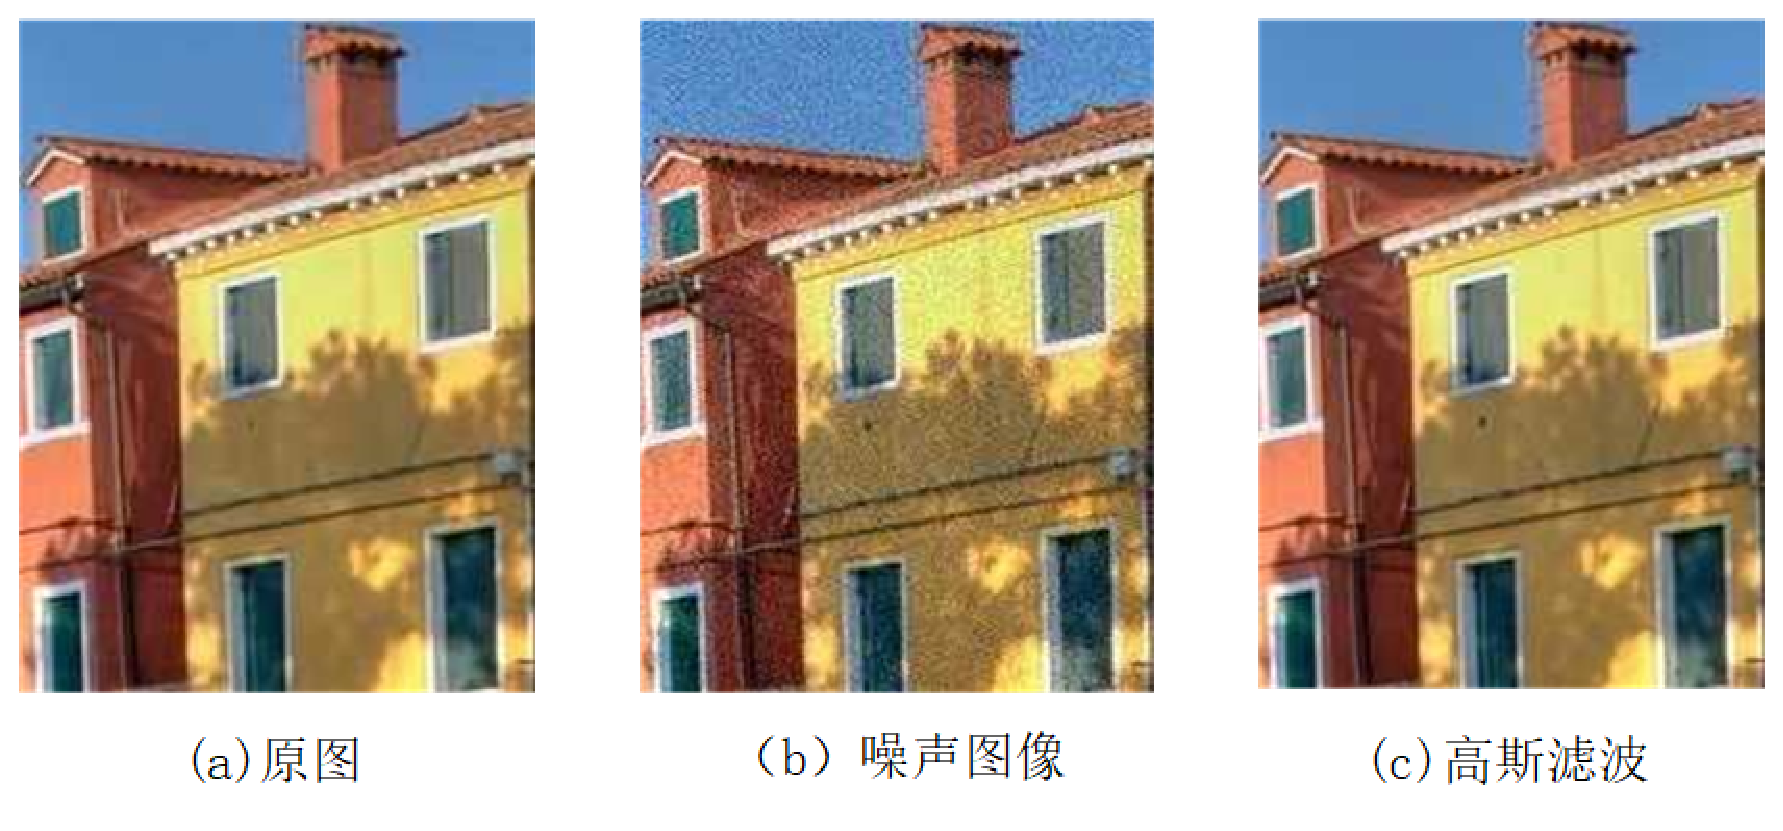
\includegraphics[height=6.63cm ,width=14.54cm]{figures/图2.1.eps}
	\caption{高斯滤波技术去噪示例}\label{图2.1}
\end{figure}

\section{本章小结}

本章是整体算法研究的前节,主要是介绍图像噪声估计方法和图像去噪方法,是视觉图像处理任务不可避免的环节,在工程应用上有极其重要的地位。噪声估计选用基于主成分分析方法的噪声强度估计技术,对图像采集设别获取的图像资源进行相应的检测,有针对的进行噪声去除,降低计算资源的消耗。由于本次研究是基于视觉图像的处理,通常是以加性高斯白噪声为主,因此不涉及乘性噪声的问题。本次研究采用的是常见的去噪方法为高斯滤波技术,凭借其计算简单的特性和可靠性,足够用于基础的视觉任务图像预处理。












